\documentclass[tikz]{standalone}
\usepackage{tikz}
\begin{document}
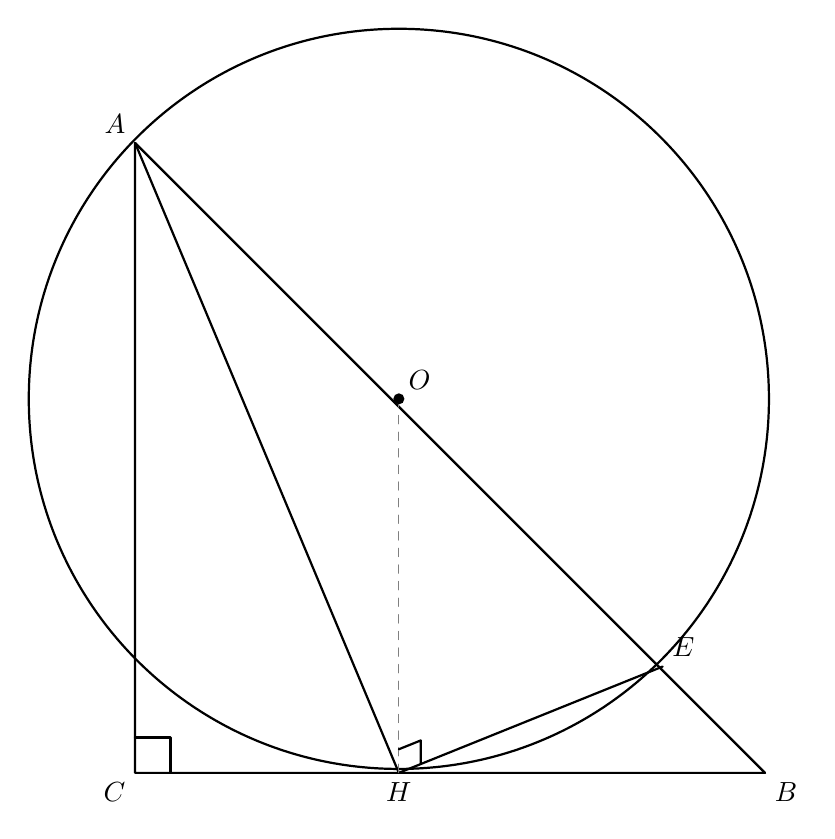
\begin{tikzpicture}[scale=1, line cap=round, line join=round]
  % Coordinates
  \coordinate (C) at (0,0);
  \coordinate (A) at (0,8);
  \coordinate (B) at (8,0);
  \coordinate (H) at (3.35,0);
  \coordinate (E) at (6.7,1.35);
  \coordinate (O) at (3.35,4.75);

  % Circle
  \draw[thick] (O) circle (4.7);

  % Triangle and segments
  \draw[thick] (A) -- (C) -- (B) -- cycle;
  \draw[thick] (A) -- (H);
  \draw[thick] (H) -- (E);
  \draw[thick] (A) -- (B);

  % Dashed radius OH
  \draw[dashed, gray] (O) -- (H);

  % Right angle marks
  \draw[thick] (0,0.45) -- (0.45,0.45) -- (0.45,0);
  \draw[thick] (3.35,0.3) -- (3.628,0.412) -- (3.628,0.112);

  % Points
  \fill (O) circle (2pt);

  % Labels
  \node[above left] at (A) {$A$};
  \node[below left] at (C) {$C$};
  \node[below right] at (B) {$B$};
  \node[below] at (H) {$H$};
  \node[above right] at (E) {$E$};
  \node[above right] at (O) {$O$};
\end{tikzpicture}
\end{document}
